\mysubsectionformatted{Cloud Computing}
\myparagraph{
    Nasce per mano del NIST (National Instituite of Standard and Technology), si tratta
    di un modello capace di garantire un accesso via rete a una vasta area di risorse
    (reti, server, applicazioni, servizi ecc...) che possono essere rilasciate con la
    minima gestione o interazione con il fornitore del servizio.
    \\
    Tra le caratteristiche principali abbiamo:
    \begin{enumerate}
        \item Capacità per un utente di registrarsi e ricevere i servizi senza dover affrontare
              lunghe attese.
        \item Capacità di accedere ai servizi mediante piattaforme standard (desktop, laptop ecc\dots)
        \item Le risorse sono messe in comune tra tutti gli utenti o clienti.
        \item Scalabilità rapida per far fronte a un grande quantitativo di utenti.
        \item La fatturazione del servizio è monitorato in base a quanto si sta usando quel servizio.
    \end{enumerate}

    \mysubsubsectionformatted{La gerarchia del Cloud}
    \vspace{-1cm}
    \begin{center}
        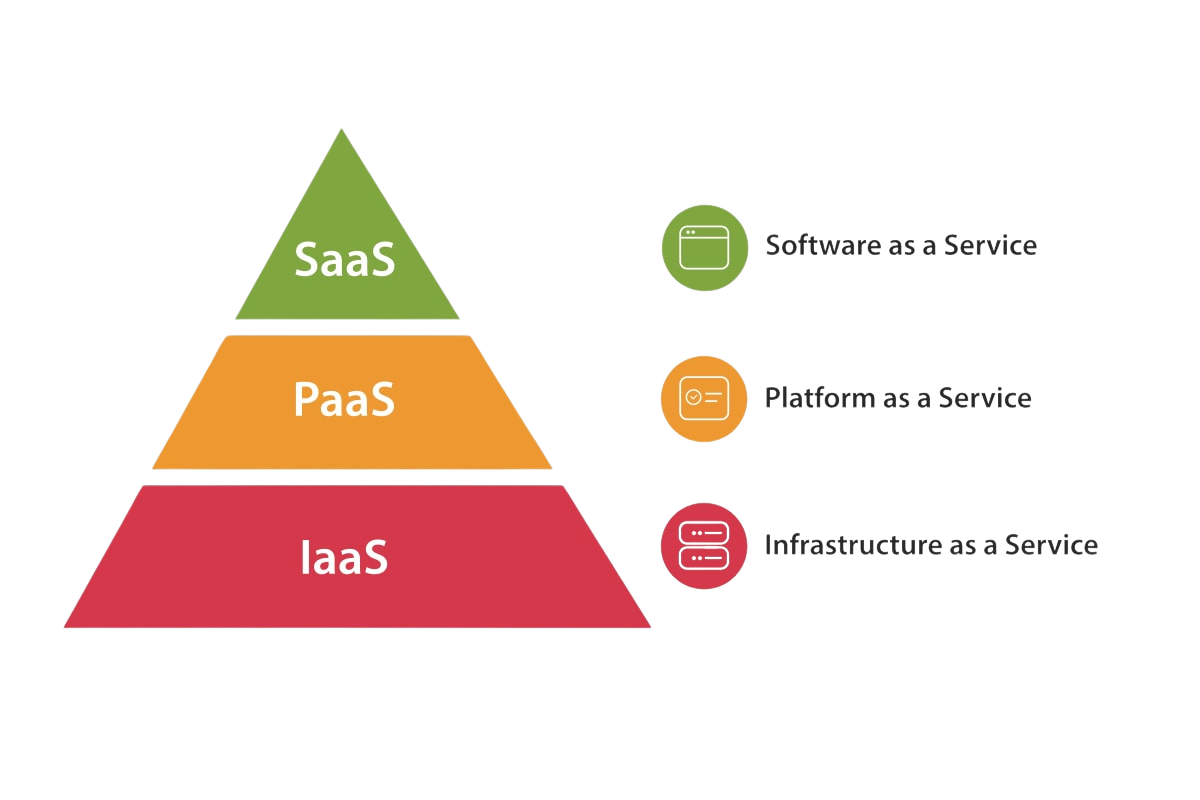
\includegraphics[width=13cm]{cloud/gerarchia_cloud.jpg}
    \end{center}

    \begin{center}
        \resizebox{\columnwidth}{!}{%
            \begin{tabular}{|l|l|}
                \hline
                \cellcolor[HTML]{009901}{\color[HTML]{FFFFFF} \textbf{SaaS}} & Applicazioni rivolte agli utenti finali, inviati tramite il web                                                                                  \\ \hline
                \cellcolor[HTML]{F56B00}{\color[HTML]{FFFFFF} \textbf{PaaS}} & \begin{tabular}[c]{@{}l@{}}Set di strumenti e servizi per creare codici e distribuire\\ le applicazioni in modo rapido e efficiente\end{tabular} \\ \hline
                \cellcolor[HTML]{CB0000}{\color[HTML]{FFFFFF} \textbf{IaaS}} & \begin{tabular}[c]{@{}l@{}}Hardware e software che da vita a tutti i servizi (server, \\ reti, sistemi operativi ecc\dots)\end{tabular}          \\ \hline
            \end{tabular}%
        }
    \end{center}
}